\begin{center}
{\large \bf \TITLE}
\end{center}

\section{Introduction}

Broadband access networks are proliferating: Over 90\% of US households
now have Internet access, and networks have become an essential part of
every home.  Video streaming already accounts for over 60\% of the peak
download bandwidth for the Internet~\cite{www-bismark};

Many academic institutions have high speed research networks (HSRNs) that support up to 400 Gbps connections to data centers and the cyber infrastructure. To enable high bandwidth transfers research networks typically rely on data transfer nodes in the DMZ. However, in our case we have built a separate and dedicated network that reaches into research labs and research offices at up to 200 Gbps with redundant connections. This allows participating researchers to conduct high bandwidth data transfers, such as sending large datasets within and across institutions, and to support  low latency research applications, such as AR/VR and robotics. Researchers from many disciplines are benefiting from these high speed low latency transfers. . Active researchers on our own HSRN include AR/VR, Physics, Chemistry, Robotics, Electrical Engineering, Multimedia and Performing Arts, and Computer Science.

On HSRNs, much of the data and code is potentially highly sensitive in nature, and can include personally identifiable information about experimental subjects, key experimental data that could be of interest to national security, and intellectual property such as code, research data and results, and papers.

Threat Model. An attacker could potentially access, exfiltrate, or disrupt (e.g., by modifying) sensitive research data and code on an HSRN or misuse the hardware connected to the network (e.g. DDNS). Such an  attack could originate from the Internet or from another host on the same network (e.g., as a result of malware’s lateral movement [cite]).

Unique Challenges. To prevent theft of intellectual property and unwanted data exfiltration, access, or disruption, network administrators typically rely on two solutions — both of which have limitations in HSRNs in general.

Challenge C1: Network administrators often use off-the-shelf commercial or open-source security appliances. While this approach is common on general enterprise networks (typically ~10 Gbps), it likely incurs significant performance overhead on HSRNs (e.g., 400 Gbps). For instance, products like intrusion detection systems (IDS) may alert after some delay. On our 400 Gbps network, every second of delays in alerts, could result in up to 50 GB of data exfiltrated. Furthermore, products like firewalls and intrusion prevention systems (IPS) inspect traffic in-line — generally fast enough for traditional networks (e.g., 10 Gbps), but too slow (or prohibitively expensive for academic applications) for the 400 Gbps HSRN in our institution, restricting the bandwidth and introducing additional latency for researchers on the network.

Challenge C2: Network administrators could manually create firewall bypasses for specific researchers. One technique, also known as Science DMZ [cite], would place scientific devices or data transfer servers on a separate high-speed network without any security checks. Although this approach places no restrictions on the bandwidth and latency, another compromised device (e.g., infected with malware while not on this network) could lead to data exfiltration on this isolated network. Alternatively, as in the HSRN at our current institution, network administrators create temporary firewall bypasses for specific use cases over predetermined periods. Researchers have to submit special requests to the network administrators regarding their proposed activities to bypass the security checks, including (but not limited to) the wall ports connected, the destination hostnames and ports, the amount of traffic, and the start/stop times. This is typically a manual process requiring efforts of both the researchers and network administrators — a likely bottleneck (sometimes in months) in a typically fast-paced and unpredictable research environment. Also, this manual process is prone to mistakes; we have seen cases where network administrators forgot to close ports in a timely manner, thus exposing the researchers to security risks.

Key Objectives. We want to make HSRNs secure without compromising the networks’ performance or the researchers’ user experience. Our proposed research aims to satisfy the following three goals:

KO1: Performance: Provide Researchers on the HSRN with access to  the unrestricted high bandwidth and low latency capacities offered by the network — thereby mitigating Challenge C1.
KO2: Usability: Require minimal efforts of researchers to access maximum network performance — thereby mitigating Challenge C2.
KO3: Security: Minimize the security risks to research data and the network presented in the Threat Model.

Proposed Technique. We plan to develop, deploy, and evaluate a usable system that lets researchers temporarily and securely bypass security appliances (e.g., intrusion prevention systems, or IPS) for specific use cases — on their own with informed decisions. This system consists of three components:

A researcher-facing dashboard [D] for researchers to specify security bypass for their devices and use cases [A].
A software-defined network [E], [B], [F] that enables [F] or disables [C] security bypass for a particular application based on the researchers’ action in [D].
A network measurement and analytics service to monitor, visualize and annotate and manage research traffic [G]. This service will also double as an IDS to catch potential mistakes by researchers in [D].

\begin{figure}[t]
    \centering
    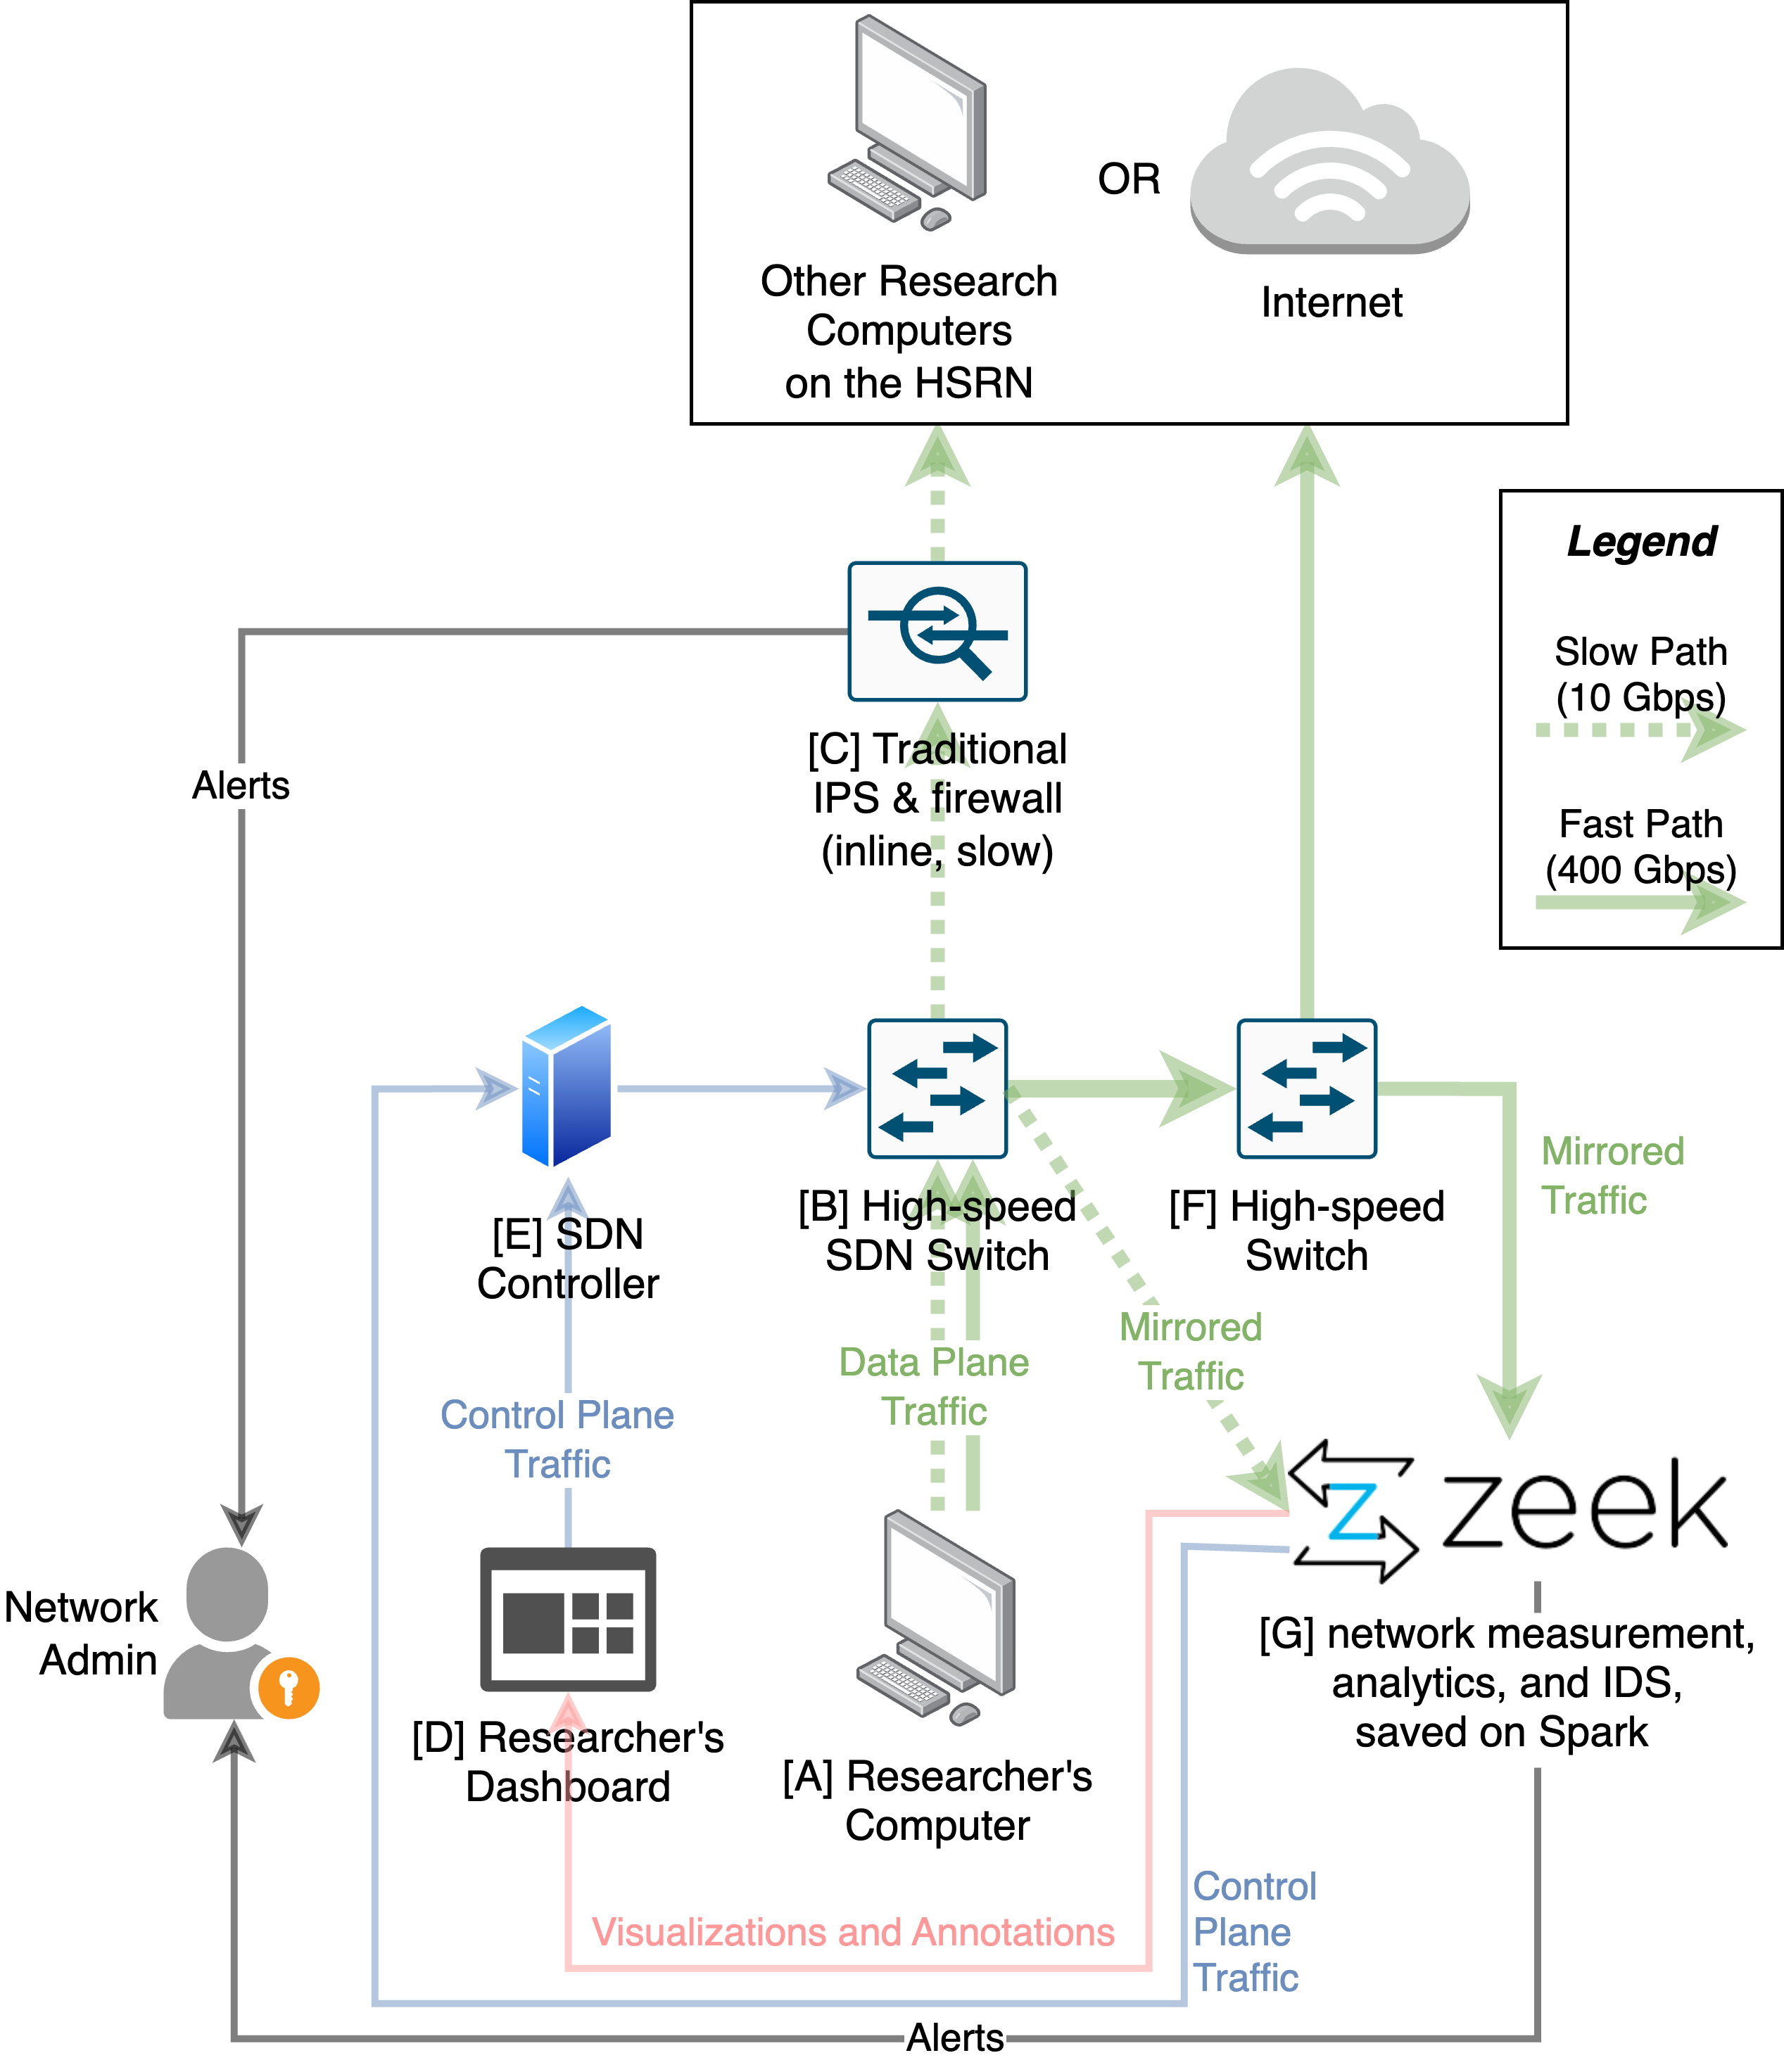
\includegraphics[width=0.5\linewidth]{figures/system.png}
    \caption{How our proposed system, including [D], [E], and [G], fits into a High Speed Research Network.}
    \label{fig:system}
\end{figure}

To illustrate how the proposed system works, we describe a sample interaction for a researcher in Figure 1. Here, a researcher connects their computer [A] to the HSRN to transfer 10 TB of data to a collaborator with the Dept of Energy (DoE). By default, all traffic, including the researchers’ normal web traffic (e.g., web, checking emails, etc.) and the data transfer with DoE, go through the secure route of the network, where all packets are inspected by traditional security appliances such as IPS. This is a slow path (from [A] through [B] to [C]) (<10 Gbps), because  typical security appliances like IPS and firewalls [C] restrict the bandwidth and increase the latency.

After the researcher begins to transfer the files to DoE, they would open the dashboard [D] — a focus of our proposed work. Here, the researcher would see traffic data reports, visualizations and annotations, based on data-driven traffic analytics at [G] (example in Figure 2). This traffic includes all network connections between [A] and the Internet, including the data transfer to DoE, along with other traffic on [A], such as web traffic. Based on the data, visualizations, and annotations, the researcher could select the DoE data transfer for security bypass for a given time or byte count (e.g., 10 TB). This action would cause the network controller [E] to automatically reroute  the existing DoE data transfer through the fast path (from [A] through [B] to [F]) (~400 Gbps) that bypasses security appliances (instead of the original slow path). The other non-DoE traffic is not affected and remains on the slow general network path.

Key Contributions. Our novelty is in the usability of the proposed approach and the ability to integrate with existing state-of-the art HSRN and security appliances. This approach will allow researchers to utilize the high bandwidth and low latency of the high-speed network ( addressing Challenge C1), in a way that is instantaneous, streamlined (addressing Challenge C2), and secure. Our proposed work focuses on achieving this usability and integration. We defer anomaly detection (e.g., identifying data exfiltration or unauthorized access) to existing literature.

Team. PI Dr. Danny Y. Huang is an Assistant Professor at NYU’s Department of Electrical and Computer Engineering. He is an expert on networking, security, and human-computer interactions. He has published papers on software-defined networking [cite], analyzing malware’s network activities [cite], visualizing network traffic for non-experts [cite], and understanding human behaviors in the context of security/privacy through user studies [cite].

Co-PI Dr. Robert Pahle is a Senior Research Scientist at NYU Research Technology. He is on the development team of NYU’s High-Speed Research Network. He is an expert on network deployment and operations, as well as open source development [cite corelink.hsrn.nyu.edu].

Co-PI: Dr. Justin Cappos is an Associate Professor at NYU’s Department of Computer Science and Engineering. He is an expert on production open source software deployments, e.g., Seattle Testbed, TUF, and in-toto [cite].

Summary. Our proposed work will benefit HSRNs at NYU and beyond, which are popular among scientists who need a high-bandwidth, low-latency computing environment. We will make HSRNs more secure and usable without compromising the networks’ performance. This simplicity promotes collaboration and innovations across disciplines, as researchers will be able to keep and share their sensitive information safely without significant administrative overhead to achieve security

// answer the following questions, and say where the reader can find the answers: Existing scientific infrastructure and distributed scientific environments that will benefit from the proposed research;How the proposed security mechanisms or infrastructure enhancements will advance scientific discoveries,collaborations, and innovations, and benefit scientific applications, users, and communities;Any unique properties of the scientific domain or infrastructure that influence the desired security functionality,design, or mechanisms; The software license that will be used for any released software, and justification for why this license has been chosen; A sustainability plan describing how the proposed system will be supported beyond the project duration; and Any ethical and operational concerns of the work, including obtaining explicit consent of target CI or entities under test, protecting the privacy of sensitive datasets, and establishing processes for informed disclosure as required.

